\documentclass[]{beamer}

\usepackage{amsthm}
\usepackage{color}
\usepackage{bussproofs}
\usepackage{float}
\usepackage{tikz}
\usepackage{setspace}
\usepackage{stmaryrd}

\usepackage{listings}
\lstset{language=Haskell}
\lstset{breaklines=true}
\lstset{basicstyle=\scriptsize\sffamily}
\lstset{frame=single}
\lstset{showstringspaces=false}
\lstset{captionpos=b}

\usetheme{uucs}

\newcommand{\functor}{<\!\!\!@\!\!\!>}
\newcommand{\bifunctor}{<\!\!\!@\!\!@\!\!\!>}

\newcommand{\W}{$\mathcal{W}$}
\newcommand{\CW}{$\mathcal{CW}$}
\newcommand{\CHW}{$\mathcal{CHW}$}

\title{Contract Inference for the Ask-Elle Programming Tutor}
\subtitle{Master thesis defense under the supervision of\\ Johan Jeuring}
\author[Beerend Lauwers]{Beerend Lauwers}

\date{26 February 2014}

\subject{Contract Inference for the Ask-Elle Programming Tutor}

\begin{document}

\frontmatter

\frame{\titlepage}

\mainmatter

\begin{frame}{Outline} \tableofcontents \note{ } \end{frame}

\section{The Ask-Elle programming tutor}

\frame{\frametitle{Ask-Elle?}

\begin{itemize}
	\item A web-based programming tutor for Haskell
	\item Developed by Alex Gerdes for his PhD
	\item Aims to help first-year CS students
\end{itemize}

How it works:

\begin{itemize}
	\item A student selects an exercise and Ask-Elle describes the goal
	\item Student writes the program \emph{incrementally}, leaving holes
	\item Ask-Elle understands the student's progress and can provide \emph{feedback}
	\item Student can ask for \emph{hints}
\end{itemize}
}

\frame{\frametitle{Screenshot of Ask-Elle interface}

\begin{center}
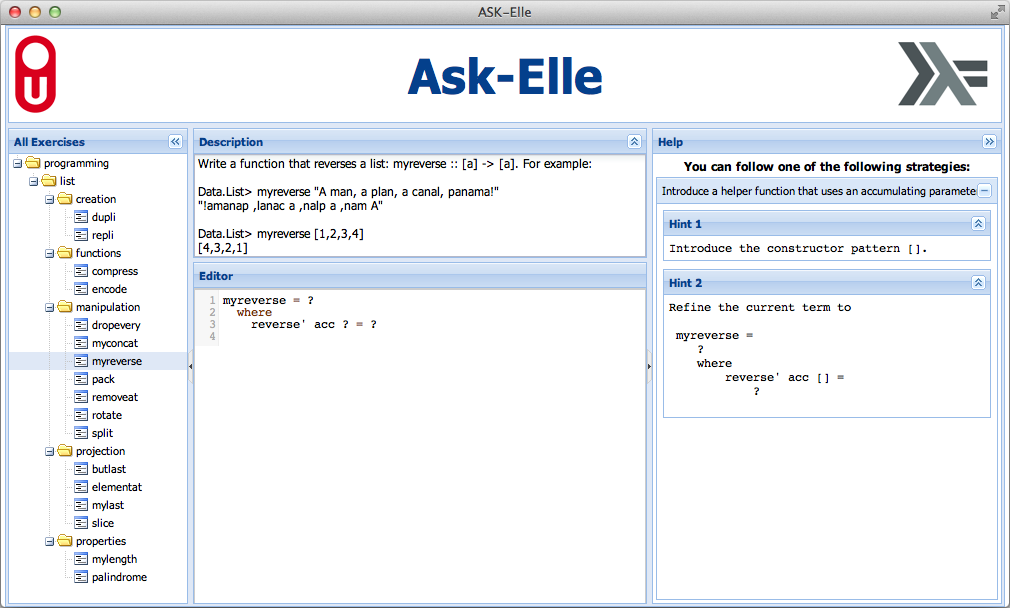
\includegraphics[scale=0.29]{fptutor.png}
\end{center}

}

\frame{\frametitle{Behind the scenes of Ask-Elle}

\begin{itemize}
	\item To define an exercise, a teacher provides \emph{model solutions}.
	\item Using \emph{strategies}, Ask-Elle compares a student's code against these model solutions
	\item If a student's code can be reduced to a model solution, Ask-Elle can provide detailed feedback and hints
	\item What happens when the student \textit{doesn't} follow a model solution?
\end{itemize}

}

\begin{frame}[fragile]
\frametitle{A gap in detailed feedback}

No model solution fits the student's solution? QuickCheck!

\begin{verbatim}
"Wrong solution: 
 range 4 6 provides a counterexample."
\end{verbatim}

Can we provide richer feedback and offer a more precise location of the programming error?

\end{frame}

\begin{frame}[fragile]
\frametitle{A gap in detailed feedback}

No model solution fits the student's solution? QuickCheck!

\begin{verbatim}
"Wrong solution: 
 range 4 6 provides a counterexample."
\end{verbatim}

Can we provide richer feedback and offer a more precise location of the programming error? \emph{Yes, with contracts!}

\end{frame}

\section{Contracts}

\frame{\frametitle{What's a contract?}

Just like its real-world counterpart, a programming contract stipulates \emph{prerequisites} and \emph{guarantees} between two parties: 
\begin{itemize}
	\item The function being called (\emph{the callee})
	\item The function receiving the result (\emph{the caller})
\end{itemize}

Simple example: the function must only accept natural numbers (\emph{a prerequisite}) and will always return natural numbers (\emph{a guarantee}).

And just like in real life, these contracts can be \emph{violated}.

}

\frame{\frametitle{Contract violations and blame assignment}

When a \emph{contract violation} occurs, blame must be assigned:
\begin{itemize}
	\item Prerequisite violation $\rightarrow$ blame is on the \emph{caller}.
	\item Guarantee violation $\rightarrow$ blame is on the \emph{callee}.
\end{itemize}

Adding contracts to your code:
\begin{itemize}
 	\item Aids in debugging 
 	\item Provides automated runtime enforcement of constraints and invariants
\end{itemize}

We use the \texttt{typed-contracts} contract library by Hinze et al.

}

\subsection{The \texttt{typed-contracts} library}

\begin{frame}[fragile]
\frametitle{Constructing a contract}

\texttt{typed-contracts} uses a GADT:

\begin{lstlisting}[mathescape]
data Contract a where
   Prop      :: (a $\rightarrow$ Bool) $\rightarrow$ Contract a
   Function  :: Contract a $\rightarrow$ (a $\rightarrow$ Contract b) $\rightarrow$ Contract (a $\rightarrowtriangle$ b)
   Pair      :: Contract a $\rightarrow$ (a $\rightarrow$ Contract b) $\rightarrow$ Contract (a, b)
   List      :: Contract a $\rightarrow$ Contract [a]
   Functor   :: Functor f $\Rightarrow$ Contract a $\rightarrow$ Contract (f a)
   Bifunctor :: Bifunctor f $\Rightarrow$ Contract a $\rightarrow$ Contract b $\rightarrow$ Contract (f a b)
   And       :: Contract a $\rightarrow$ Contract a $\rightarrow$ Contract a
\end{lstlisting}

\end{frame}

\begin{frame}[fragile]
\frametitle{Constructing a contract - \texttt{Prop} constructor}

\begin{lstlisting}[mathescape]
Prop :: (a $\rightarrow$ Bool) $\rightarrow$ Contract a
\end{lstlisting}

\begin{itemize}
	\item Lift a function to a contract
	\item Defines a constraint or property on a value
\end{itemize}

\end{frame}

\begin{frame}[fragile]
\frametitle{Constructing a contract - \texttt{Function} constructor}

\begin{lstlisting}[mathescape]
Function :: Contract a $\rightarrow$ (a $\rightarrow$ Contract b) $\rightarrow$ Contract (a $\rightarrowtriangle$ b)
\end{lstlisting}

\begin{itemize}
	\item Defines a dependent function contract
	\item Note the $\rightarrowtriangle$
\end{itemize}

\end{frame}

\begin{frame}[fragile]
\frametitle{Constructing a contract - \texttt{Pair} constructor}

\begin{lstlisting}[mathescape]
Pair :: Contract a $\rightarrow$ (a $\rightarrow$ Contract b) $\rightarrow$ Contract (a, b)
\end{lstlisting}

\begin{itemize}
	\item Defines a dependent pair
	\item Not used in this presentation
\end{itemize}

\end{frame}

\begin{frame}[fragile]
\frametitle{Constructing a contract - \texttt{List} constructor}

\begin{lstlisting}[mathescape]
List :: Contract a $\rightarrow$ Contract [a]
\end{lstlisting}

\begin{itemize}
	\item Lifts contracts to the list level
\end{itemize}

\end{frame}

\begin{frame}[fragile]
\frametitle{Constructing a contract - \texttt{Functor} constructor}

\begin{lstlisting}[mathescape]
Functor :: Functor f $\Rightarrow$ Contract a $\rightarrow$ Contract (f a)
\end{lstlisting}

\begin{itemize}
	\item A container type that can house types of kind $* \rightarrow *$
	\item Examples: \texttt{Maybe}, \texttt{Just}
\end{itemize}

\end{frame}

\begin{frame}[fragile]
\frametitle{Constructing a contract - \texttt{Bifunctor} constructor}

\begin{lstlisting}[mathescape]
Bifunctor :: Bifunctor f $\Rightarrow$ Contract a $\rightarrow$ Contract b $\rightarrow$ Contract (f a b)
\end{lstlisting}

\begin{itemize}
	\item A container type that can house types of kind $* \rightarrow * \rightarrow *$
	\item Examples: \texttt{Either}, 2-tuple
\end{itemize}

\end{frame}

\begin{frame}[fragile]
\frametitle{Constructing a contract - \texttt{And} constructor}

\begin{lstlisting}[mathescape]
And :: Contract a $\rightarrow$ Contract a $\rightarrow$ Contract a
\end{lstlisting}

\begin{itemize}
	\item Chains contracts together
	\item All contracts are asserted when a value is provided
\end{itemize}

\end{frame}

\begin{frame}[fragile]
\frametitle{Some notation for contracts}

\begin{lstlisting}[mathescape]
c$_1$ $\rightarrowtriangle$ c$_2$		= Function c$_1$ (const c$_2$)
(&)		= And
c$_1$ $\functor$ c$_2$		= c$_1$ & Functor c$_2$
c$_1$ $\bifunctor$ (c$_2$,c$_2$)	= c$_1$ & Bifunctor c$_2$ c$_3$
\end{lstlisting}

\begin{itemize}
	\item \texttt{c$_1$ $\rightarrowtriangle$ c$_2$} defines a non-dependent function contract
	\item \texttt{$\functor$} and \texttt{$\bifunctor$} use \texttt{c$_1$} as a contract that must hold on the container in its entirety: an \emph{outer contract}.
	\item Example: an ordered list
\end{itemize}

\end{frame}

\begin{frame}[fragile]
\frametitle{Constructing a contract: examples}

Fundamental contracts:

\begin{lstlisting}[mathescape]
true, false :: Contract a
true  = Prop ($\lambda$_ $\rightarrow$ True)
false = Prop ($\lambda$_ $\rightarrow$ False)
\end{lstlisting}

A contract that only allows natural numbers:

\begin{lstlisting}[mathescape]
nat :: Contract Int
nat = Prop ($\lambda$i $\rightarrow$ i $\geq$ 0)
\end{lstlisting}

\end{frame}

\begin{frame}[fragile]
\frametitle{Asserting contracts}

To attach a contract to a function, we use \texttt{assert}:

\begin{lstlisting}[mathescape]
assert :: String $\rightarrow$ Contract a $\rightarrow$ a $\rightarrow$ a
\end{lstlisting}

\texttt{assert} acts as a \emph{partial identity} function: in the case of a contract violation, an exception is thrown. Otherwise, it acts as identity.

\end{frame}

\begin{frame}[fragile]
\frametitle{Asserting contracts: an example}

\begin{lstlisting}[mathescape]
assert :: String $\rightarrow$ Contract a $\rightarrow$ a $\rightarrow$ a
\end{lstlisting}

\begin{lstlisting}[mathescape]
inc :: Int $\rightarrowtriangle$ Int
inc = assert "inc" (nat $\rightarrowtriangle$ nat) (fun ($\lambda$n $\rightarrow$ 1 + n))
\end{lstlisting}

\begin{itemize}
	\item \texttt{(nat $\rightarrowtriangle$ nat)} is of type \texttt{Contract (Int $\rightarrowtriangle$ Int)}
	\item So, \texttt{a} must be of type \texttt{(Int $\rightarrowtriangle$ Int)}
	\item \texttt{fun} lifts a single argument to the contract level:
\end{itemize}

\begin{lstlisting}[mathescape]
fun :: (a $\rightarrow$ b) $\rightarrow$ (a $\rightarrowtriangle$ b)
\end{lstlisting}

\end{frame}

\begin{frame}[fragile]
\frametitle{Asserting contracts: an example}

\begin{lstlisting}[mathescape]
inc :: Int $\rightarrowtriangle$ Int
inc = assert "inc" (nat $\rightarrowtriangle$ nat) (fun ($\lambda$n $\rightarrow$ 1 + n))
\end{lstlisting}

We use \texttt{app} to apply values to a \emph{contracted function} such as \texttt{inc}:

\begin{lstlisting}[mathescape]
app :: (a $\rightarrowtriangle$ b) $\rightarrow$ Int $\rightarrow$ a $\rightarrow$ b
\end{lstlisting}

It also labels the application with a number, used in feedback:
\begin{verbatim}
> app inc 1 5
> 5
> app inc 1 (-5)
> *** Exception: contract failed: the expression 
                 labeled `1' is to blame.
\end{verbatim}

\end{frame}

\section{Contract inference}

\begin{frame}[fragile]
\frametitle{Inferring contracts?}

\begin{itemize}
	\item Jurri\"en Stutterheim describes a way to \emph{infer} contracts for the components of a function in his thesis.
	\item Developed a contract inference algorithm: Algorithm \CW
	\item Based on Algorithm \W ~by Damas and Milner
	\item Works on a small let-polymorphic lambda calculus
\end{itemize}

Three requirements for contract inference:

\begin{itemize}
	\item Infer a well-typed contract for every component of a program
	\item Inferred contracts must allow a (non-strict) subset of the values allowed by the types
	\item The most general inferred contract must never fail an assertion
\end{itemize}

\end{frame}

\begin{frame}[fragile]
\frametitle{An intermediate contract grammar}

\begin{lstlisting}[mathescape]
$c$ ::=   $\rho_{\alpha}$
    |  $true_{\alpha}$
    |  $false_{\alpha}$
    |  $c_{\alpha} \rightarrowtriangle c_{\beta}$
    |  $c_{\alpha} \functor c_{\beta}$
    |  $c_{\alpha} \bifunctor (c_{\beta}, c_{\gamma})$
    (...)
    
$\sigma$ ::=   $c$
    |  $\forall{true_{\alpha}}.\sigma$
\end{lstlisting}

\begin{itemize}
	\item Contract grammar is library-agnostic
	\item They must be translated to a contract library of choice
	\item Instead of fresh type variables, you have fresh \textit{contract} variables
\end{itemize}

\end{frame}

\begin{frame}[fragile]
\frametitle{Examples of inferred contracts}

\begin{itemize}
	\item Function: \texttt{id :: a $\rightarrow$ a}
	\item Contract: \texttt{$true_1$ $\rightarrowtriangle$ $true_1$}
\end{itemize}

\begin{itemize}
	\item Function: \texttt{const :: a $\rightarrow$ b $\rightarrow$ a}
	\item Contract: \texttt{$true_1$ $\rightarrowtriangle$ $true_2$ $\rightarrowtriangle$ $true_1$}
\end{itemize}

\begin{itemize}
	\item Function: \texttt{map :: (a $\rightarrow$ b) $\rightarrow$ [a] $\rightarrow$ [b]}
	\item Contract: \texttt{($true_1$ $\rightarrowtriangle$ $true_2$) $\rightarrowtriangle$ ($true_3$ $\functor$ $true_1$) $\rightarrowtriangle$ ($true_4$ $\functor$ $true_2$)}
\end{itemize}

\end{frame}

\begin{frame}[fragile]
\frametitle{Stutterheim's goal: superior feedback in Ask-Elle}

\begin{itemize}
	\item If a student's code does not follow a model solution, the only feedback possible is a QuickCheck counterexample
	\item Stutterheim wanted to express the QuickCheck properties as a contract for the main function
	\item Then use contract inference to infer contracts for the rest of the code
	\item Generate code that annotates all function applications with contract assertations
	\item Finally, apply the counterexample to the annotated code
	\item A contract violation occurs and offers a more precise location for the programming error
\end{itemize}

\end{frame}

\section{Expanding on Stutterheim's work}

\begin{frame}[fragile]
\frametitle{Limitations present in Stutterheim's system}

We address:
\begin{itemize}
	\item A system for code generation is left implicit
	\item Substitutions generated by Algorithm \CW ~are placed in a global set, which may result in generating an inferred contract that causes a violation during assertion
\end{itemize}

We do \textit{not} address:

\begin{itemize}
	\item Inability of Algorithm \CW ~to handle dependent contracts
	\item Lack of constant expression contracts
	\item Full integration with the Ask-Elle programming tutor
\end{itemize}

\end{frame}

\begin{frame}[fragile]
\frametitle{Our contributions}

\begin{itemize}
	\item We extend the contract inference algorithm to the Ask-Elle syntax, based on Helium, producing Algorithm \CHW
	\item Before performing contract inference, we perform AST transformations to simplify contract inference
	\item We generate \textit{initial contracts} that simplify contract inference even further, especially in the case of mutually recursive functions
	\item Substitutions are divided into two lists: global and local, avoiding the aforementioned contract violation problem
	\item We provide a system to generate code for the \textit{typed-contracts} library
\end{itemize}

\end{frame}

\subsection{System overview}

\subsection{AST transformations}

\subsection{Type source}

\subsection{Contract inference}

\subsection{Code generation}

\subsection{Generation of final contracts}

\section{Results}

\section{Future work}

\section{Conclusions}

\section*{Questions?}

\end{document}